\documentclass[12pt]{article}

\usepackage{graphicx}
\graphicspath{ {figures/} }
\usepackage[left=1.5cm,right=1cm,top=1.5cm,bottom=2cm]{geometry}


\usepackage[utf8]{inputenc}
\usepackage{t1enc}
\usepackage[magyar]{babel}
\linespread{1.0}

\usepackage{footnote}
\usepackage{subfigure}
\usepackage{float}
\usepackage{pdfpages}

\title{
	{Digitális jelfeldolgozás vizsga}\\
	{\large Sapientia\\
	Erdélyi Magyar Tudományegyetem, Marosvásárhely}
}
\author{Patka Zsolt-András}
\date{2020}

%%%%%%%%%%%%%%%%%%%%%%%%%%%%%%%%%%%%%%%%%%%%%%%%%%%%%%%%%%%%%%%%%%%%%%%%%
\begin{document}

\maketitle
\pagenumbering{gobble}

\tableofcontents
\listoffigures

\pagenumbering{arabic}
\section{Feladatok}
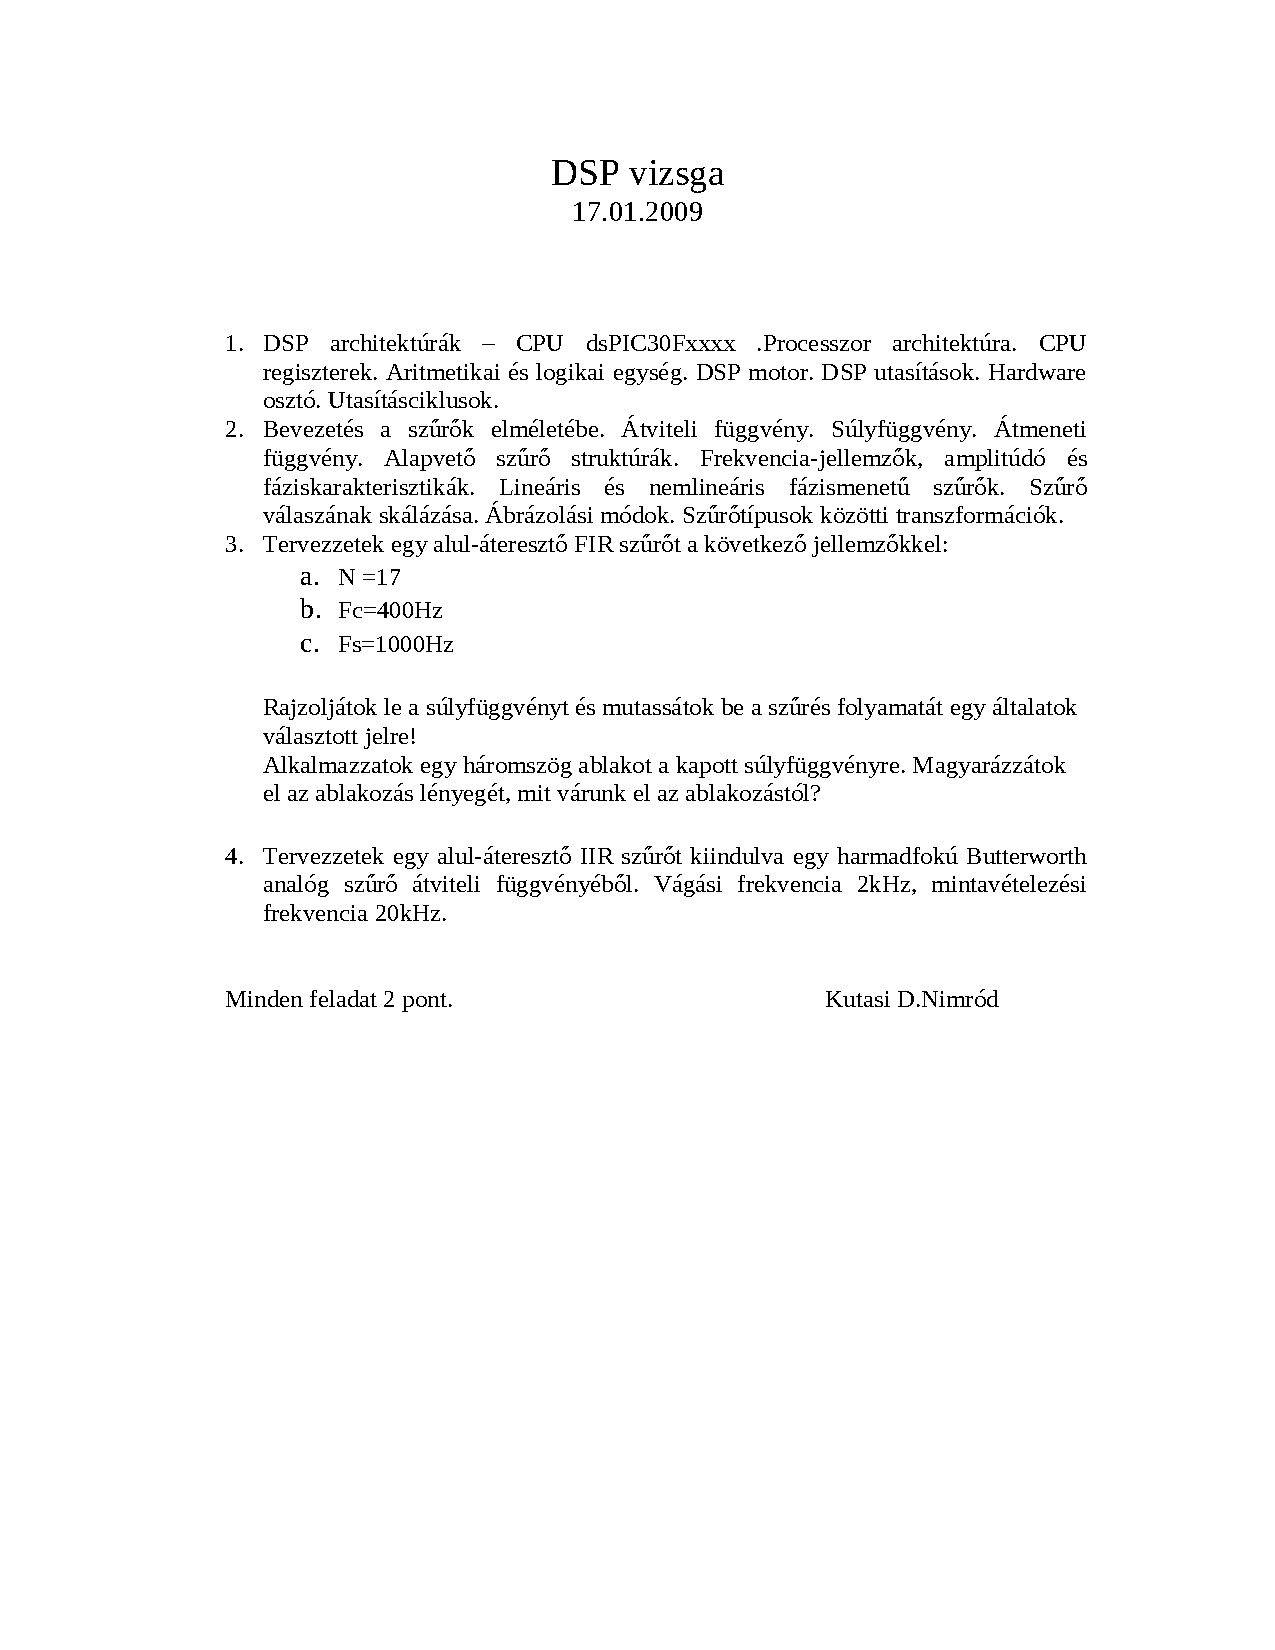
\includepdf[pages={1}]{DSPvizsga_Patka.pdf}

\section{1. Feladat}
\subsection{DSP architektúrák}

A digitális jelprocesszor (DSP) egy mikroszámítógép kibővített központi egysége. A kibővítés lehetővé teszi a műveletek gyorsabb végrehajtását és a párhuzamos művelet elvégzést, mint például: hardveres szorzás, MAC művelet (szorzás és összeadás egy utasításciklus alatt), hardveres eltolás.

A mikroprocesszoroknál két fajta architektúra lehetséges: Neumann és Harvard. A dsPIC-ek a Harvard architektúrát (pontosabban módosított Harvard) használják ami azt jelenti, hogy a programmemória és az adatmemória külön van választva. Neumann architektúra esetén egy helyen van a programmemória az adatmemóriával. A módosítás a Harvard architektúrán az, hogy a programmemória egy része használható adatmemóriaként (ezt hívják PSV - Program Space Visibility technikának).

A dsPIC jellegzetessége, hogy az adatmemória két részre van osztva: X és Y memóriára. Ez azért volt megvalósítva, mert így egyidőben lehet két adattal dolgozni.

\subsection{Processzor architektúra}

\begin{figure}[H]
    \centering
    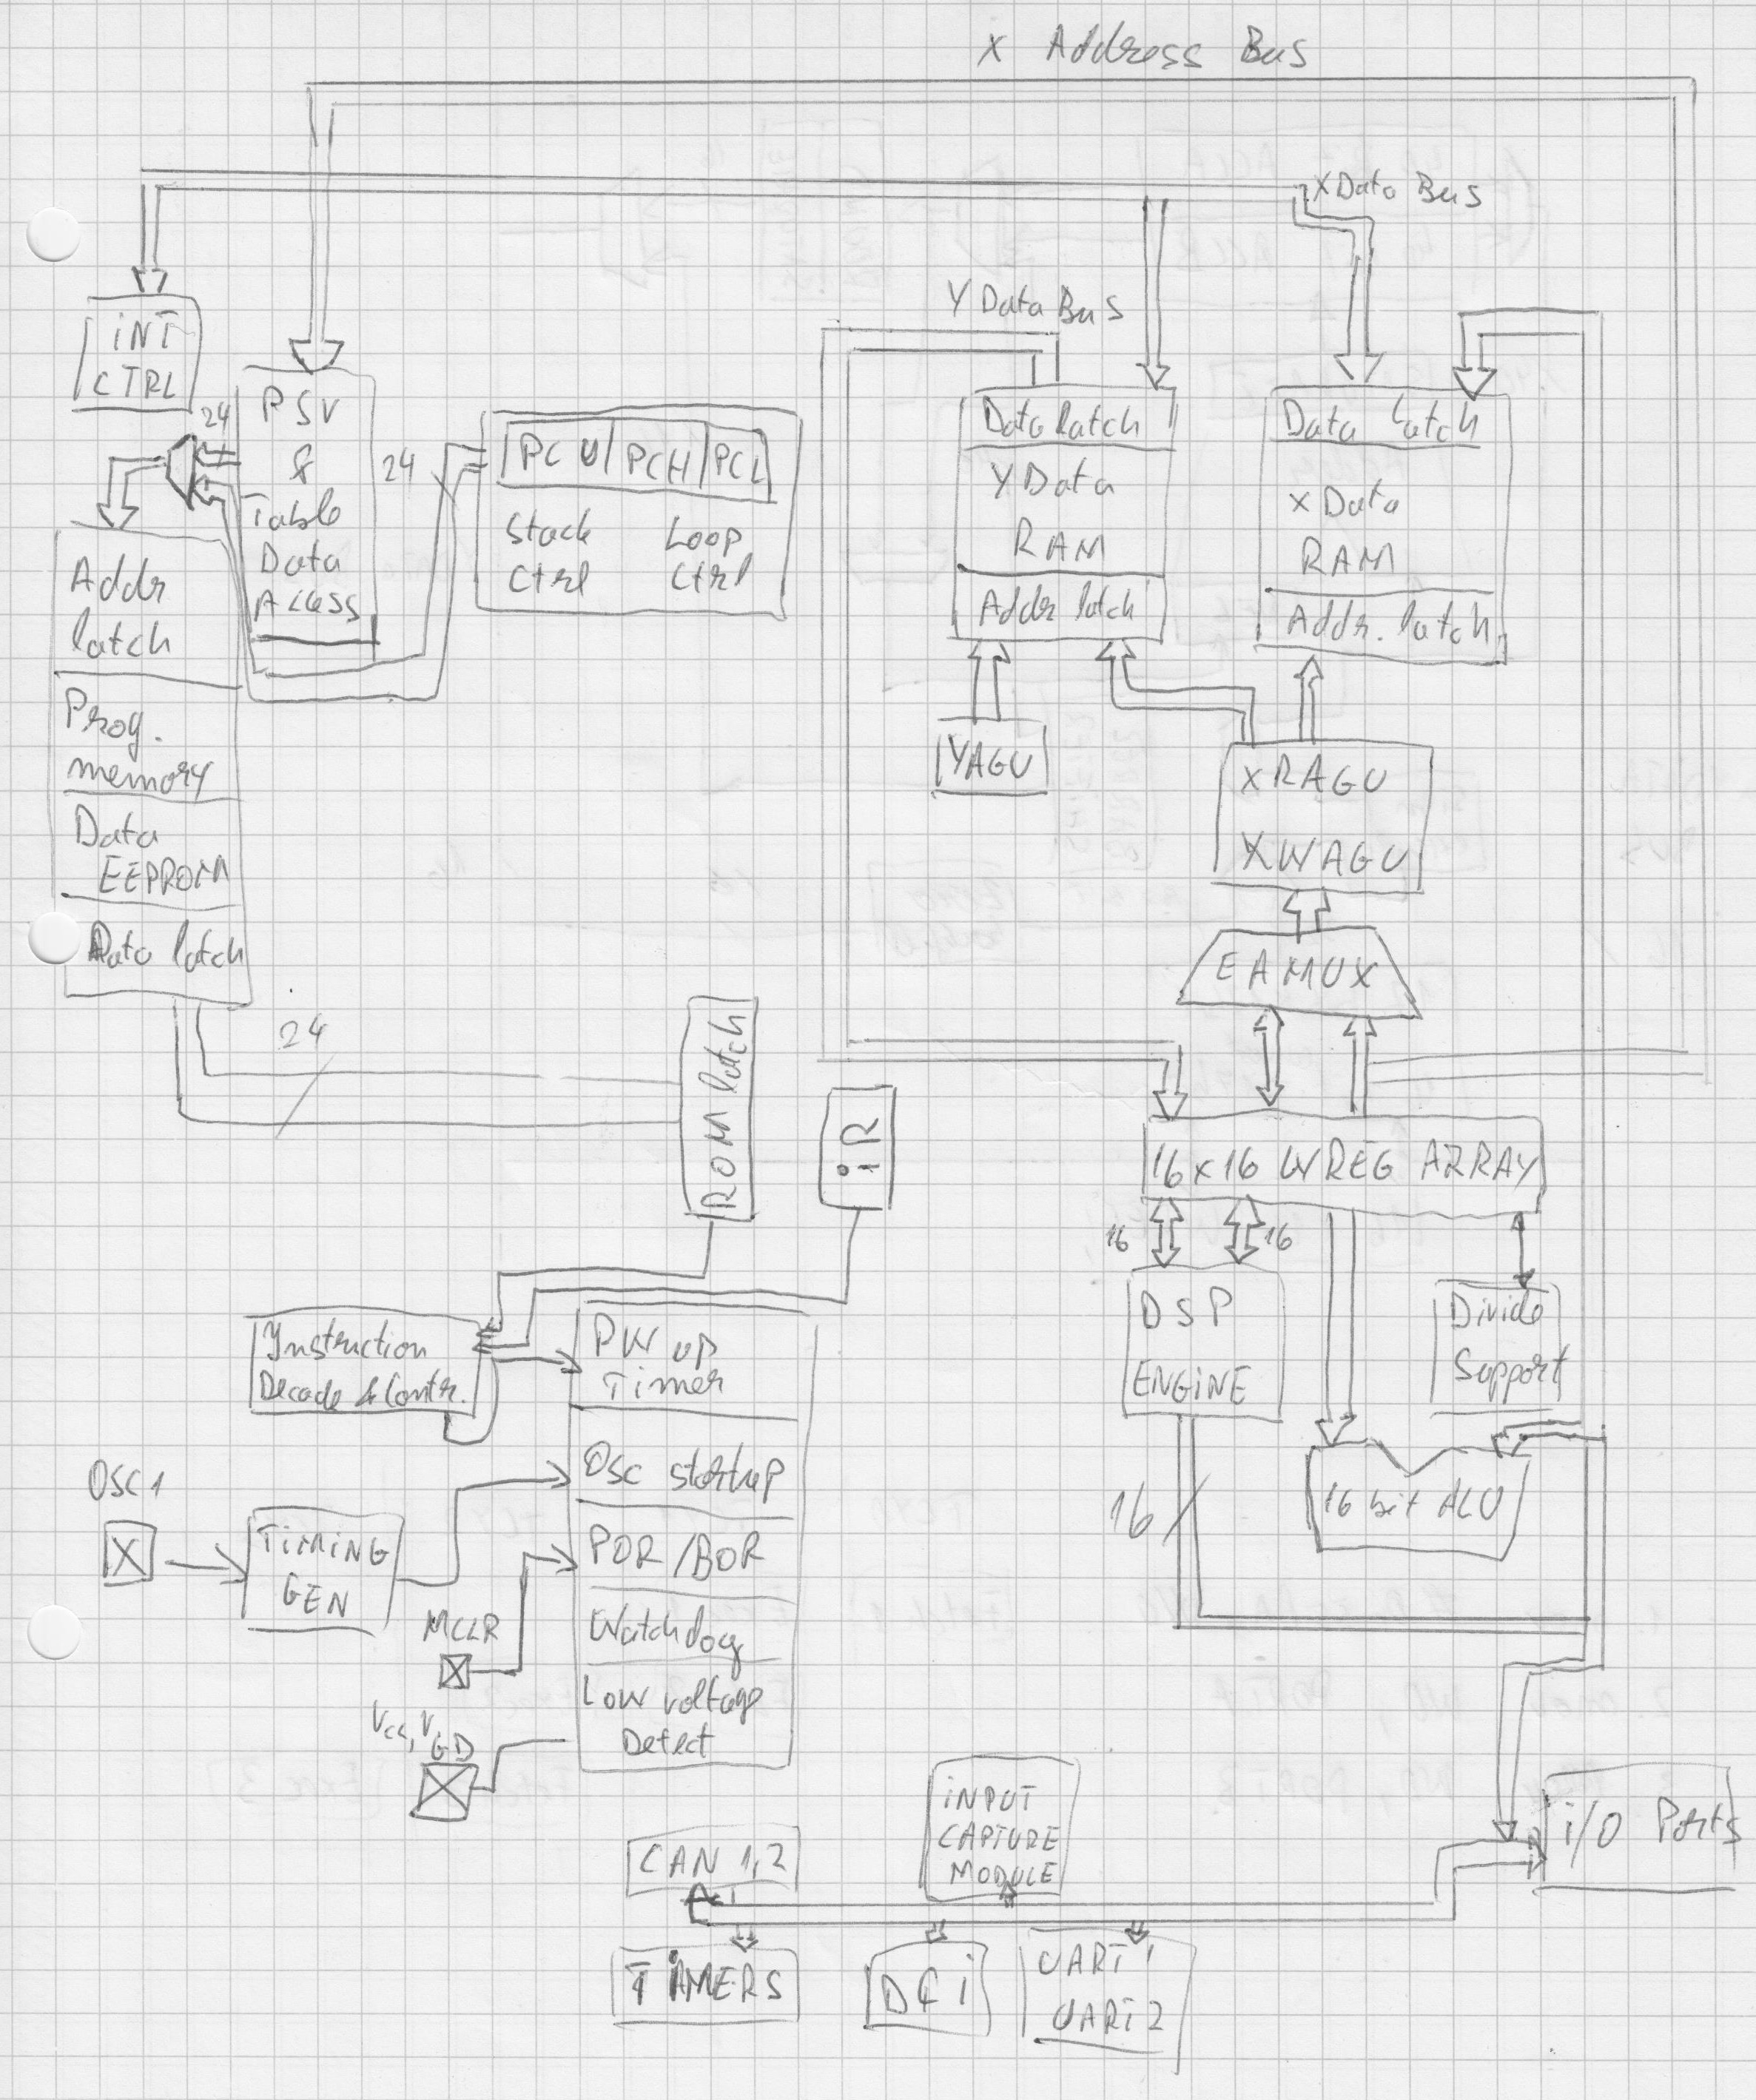
\includegraphics[scale=0.13]{figures/dsp_cpu.jpg}
    \caption{Processzor architektúra}
\end{figure}

\subsection{CPU regiszterek}

Fontosabb regiszterek:

\begin{itemize}
    \item W4, W5, W6, W7 - operandus regiszterek
    \item W8, W9, W10, W11 - címregiszterek (W8 és W9 - X memóriának, W10 és W11 - Y memóriának)
    \item W14 - frame pointer
    \item W15 - stack pointer
    \item CORCON - CPU viselkedését módosító flag-eket tartalmazó regiszter
    \item ACCA és ACCB - 40 bites akkumulátorok (3 darab 16 bites regiszterben vannak eltárolva)
\end{itemize}

\subsection{Aritmetikai és logikai egység}

Az ALU (Arithmetic Logic Unit) képes összeadást, kivonást, logikai műveleteket és egybites eltolást elvégezni. Az operandusokat a W regiszterekből vagy az adatmemóriából jönnek, az eredmény kerülhet ugyancsak a W regiszterbe vagy az adatmemóriába. 

\subsection{DSP motor}

A DSP motor viselkedését a CORCON regiszter bitjeit állítva tudjuk módosítani:

\begin{itemize}
    \item IF: egész vagy törtszámos szorzást végezzen
    \item US: előjeles vagy előjel nélküli számokkal dolgozzon
    \item SATA: legyen A regiszterre telítés vagy sem
    \item SATB: legyen a B regiszterre telítés vagy sem
\end{itemize}

\begin{figure}[H]
    \centering
    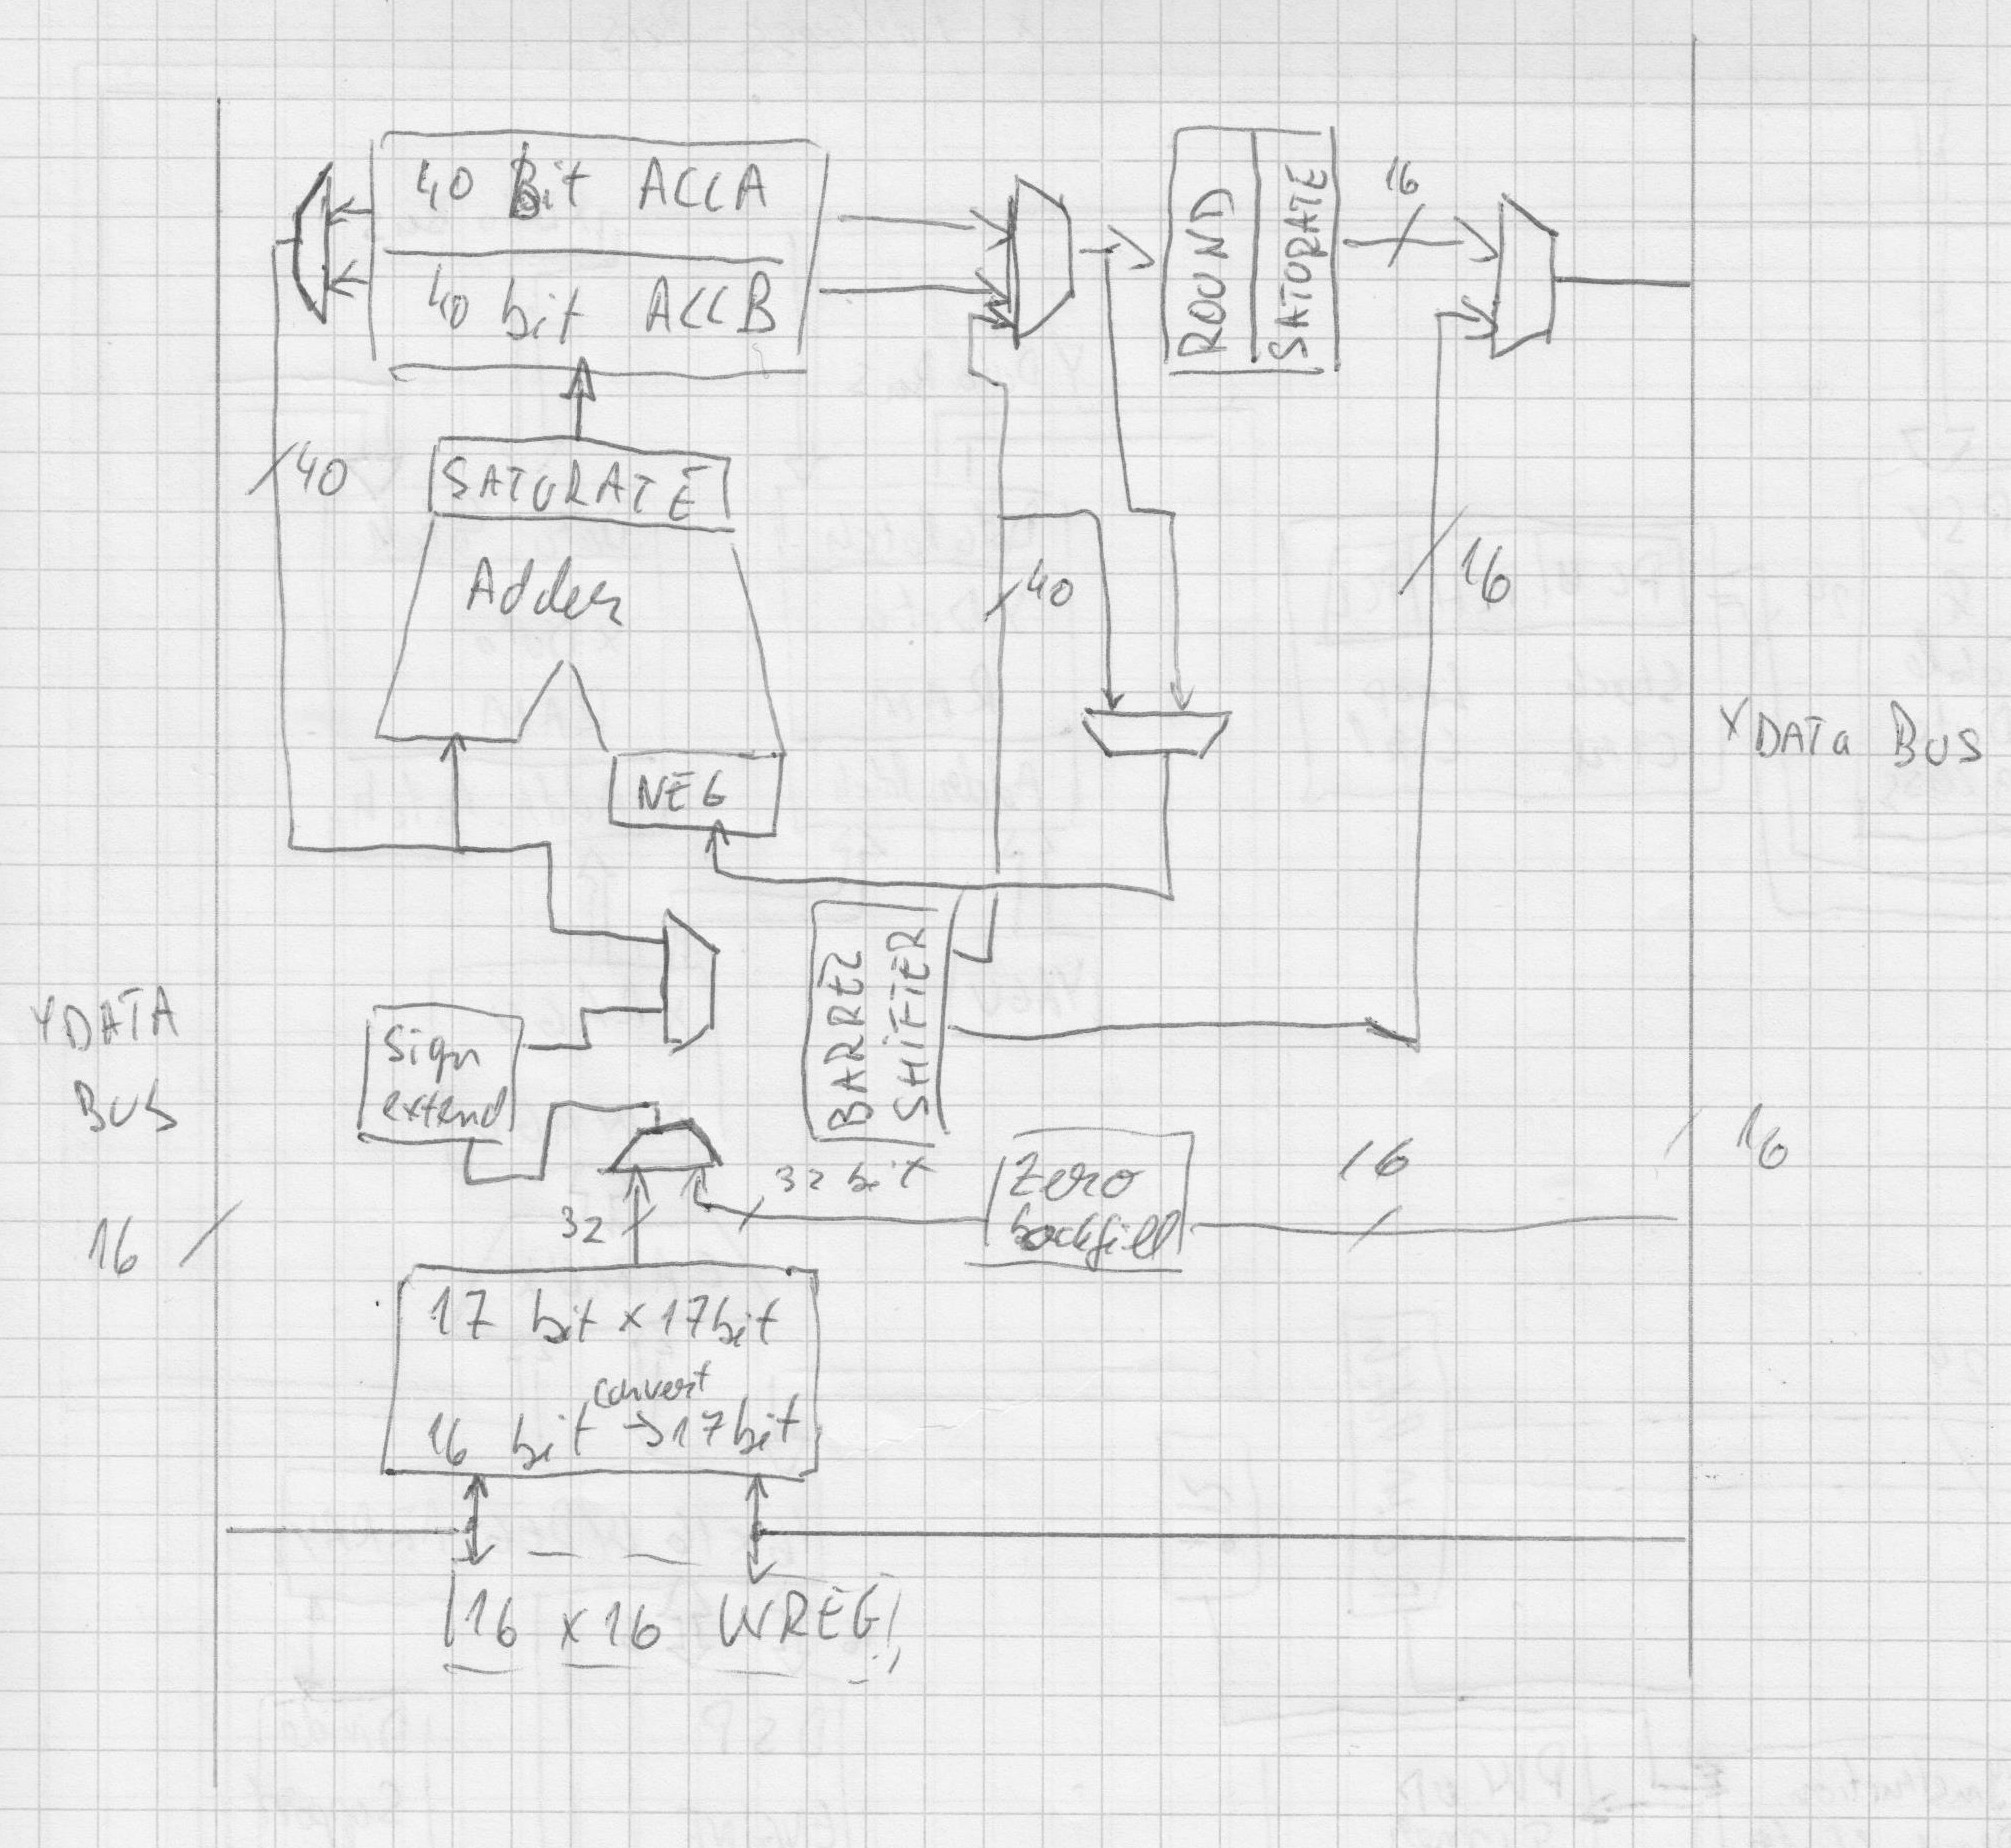
\includegraphics[scale=0.15]{figures/dsp_engine.jpg}
    \caption{DSP motor}
\end{figure}

\subsection{DSP utasítások}

\begin{itemize}
    \item mac: $a = a + b * c$ (multiply and accumulate)
    \item msc: $a = a - b * c$ (multiply and subtract)
    \item mpy: $a = b * c$ (multiply)
    \item mpy.n: $a = - b * c$ (multiply and negate)
    \item ed: $a = (b - c) ^ 2$ (euclidean distance)
    \item edac: $a = a + (b - c) ^ 2$ (euclidean distance and accumulate)
\end{itemize}

Példa: MAC W4*W5, A, [W8]+=2, W4, [W10]+=2, W5

Itt W4*W5 $\rightarrow$ A, [W8]+2 $\rightarrow$ W4, [W10]+2 $\rightarrow$ W5. Fontos, hogy a harmadik operandus (itt [W8]) X memóriát címző regiszter legyen és az ötödik operandus (itt [W10]) Y memóriát címző regiszter.

\subsection{Hardware osztó}

A dsPIC30F-nél az osztó blokk képes előjeles és előjel nélküli egész számok osztására. Az osztás hányadosa a W0 regiszterbe kerül és a maradék a W1-es regiszterbe. Műveletek:

\begin{itemize}
    \item DIVF: 16/16 előjeles törtszám osztás
    \item DIV.SD: 32/16 előjeles osztás
    \item DIV.UD: 32/16 előjel nélküli osztás
    \item DIV.UW: 16/16 előjel nélküli osztás
\end{itemize}

\subsection{Utasításciklusok}

A dsPIC-ek pipeline-ozott architektúrát használnak, amiből kifolyólag az egymás után követő utasítások nem kell megvárják amíg az azelőtti utasítás minden fázisa véghez ment (Fetch és Execute), hanem amíg az első utasítás az execute fázisban van, addig a második utasítás lehet a fetch fázisban. Ez gyorsításhoz és az erőforrások hatékonyabb kihasználásához vezet.

\begin{figure}[H]
    \centering
    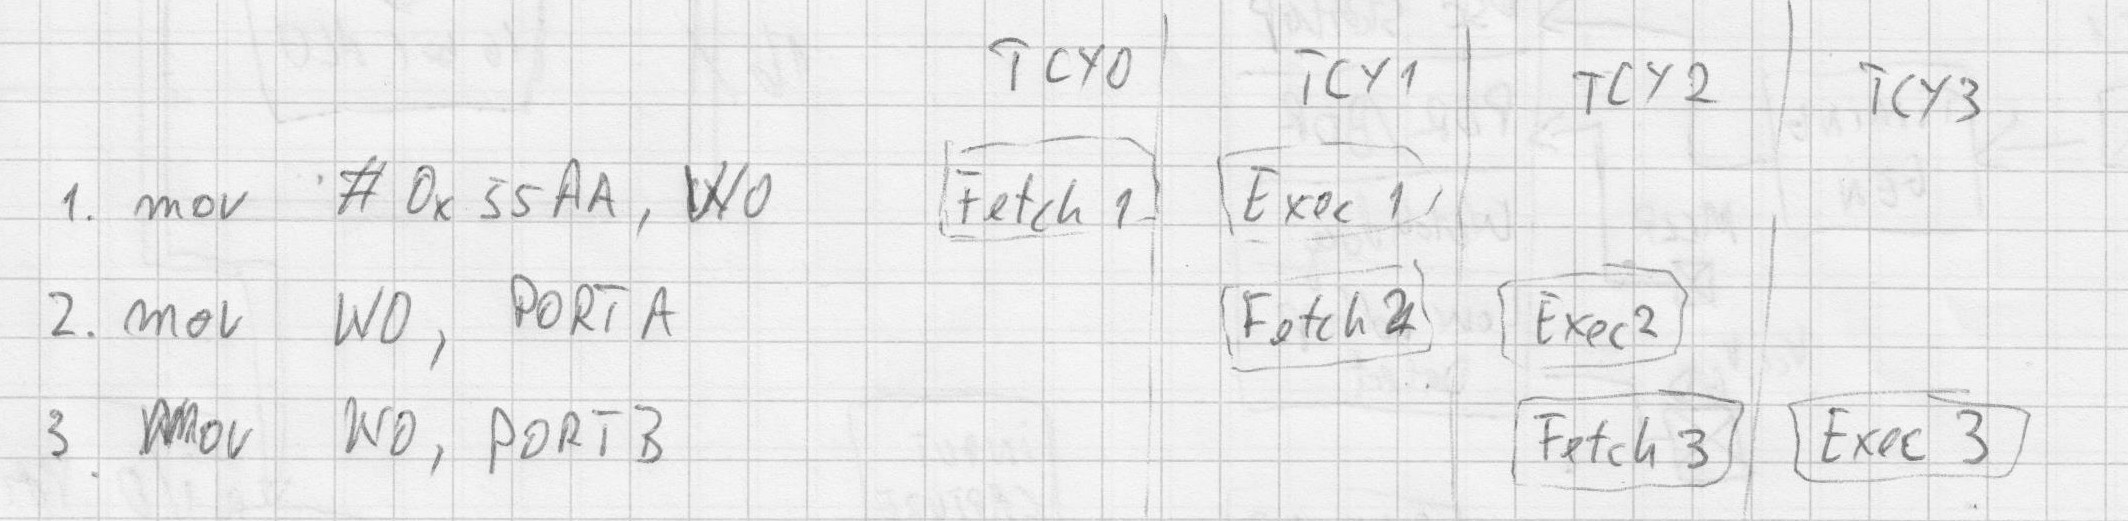
\includegraphics[scale=0.25]{figures/dsp_fetch_ex.jpg}
    \caption{Utasításciklusok}
\end{figure}


\section{2. Feladat}
\subsection{Szűrők - elméleti áttekintés}

Szűrés által csillapítani (kiszűrni) tudjuk a jelekből a nem kívánt frekvencia komponenseket úgy, hogy a számunkra fontos frekvencia komponenseket változatlanul átengedjük.

\subsection{Átviteli függvény}

Egy szűrőt megadhatunk egy átviteli függvény segítségével. Az átviteli függvény adja meg a rendszer kimenetei és bemenetei közötti összefüggést. 

A szűrés történhet úgy, hogy a jelet átvisszük a frekvencia tartományba (Fourier transzformált), összeszorozzuk az átviteli függvénnyel és ezután visszavisszük az időtartományba (Inverz Fourier transzformált). Egy másik lehetőség (FIR szűrő), hogy az átviteli függvénynek elvégezzük az inverz Fourier transzformáltját, így a szűrés csak egy egyszerű konvolúció a bemeneti jel és a súlyfüggvény között (a frekvencia tartományban szorzás megfelel az időtartományban a konvolúcióval).

\subsection{Szűrő struktúrák}

Több fajta szűrő létezik:

\begin{itemize}
    \item Alul-áteresztő
    \item Felül-áteresztő
    \item Sávzáró
    \item Sáváteresztő
    \item Mindent áteresztő (fázist változtatja meg, például sztereó hangzás eléréséért)
\end{itemize}

\begin{figure}[H]
    \centering
    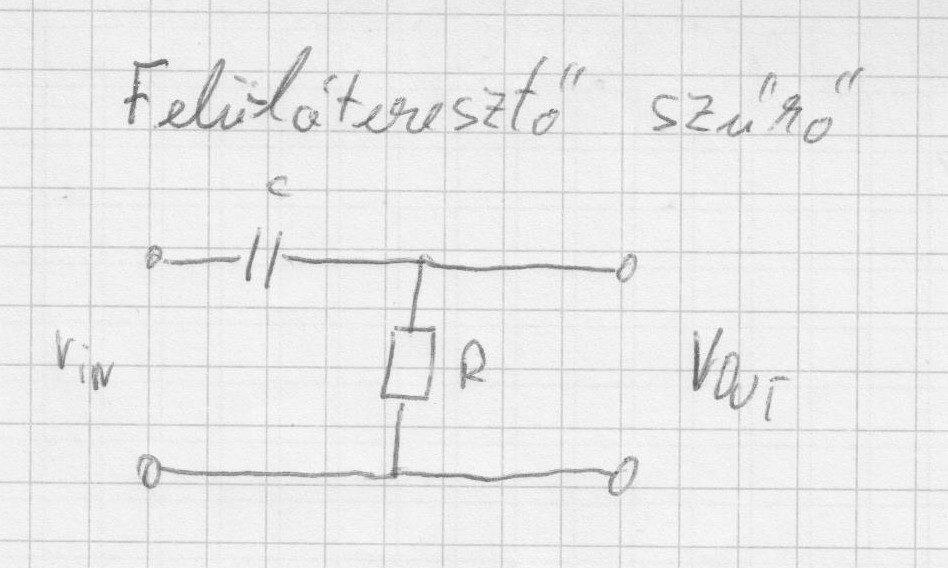
\includegraphics[scale=0.25]{figures/szuro_hp_rc.jpg}
    \caption{Felül-áteresztő szűrő}
\end{figure}

\begin{figure}[H]
    \centering
    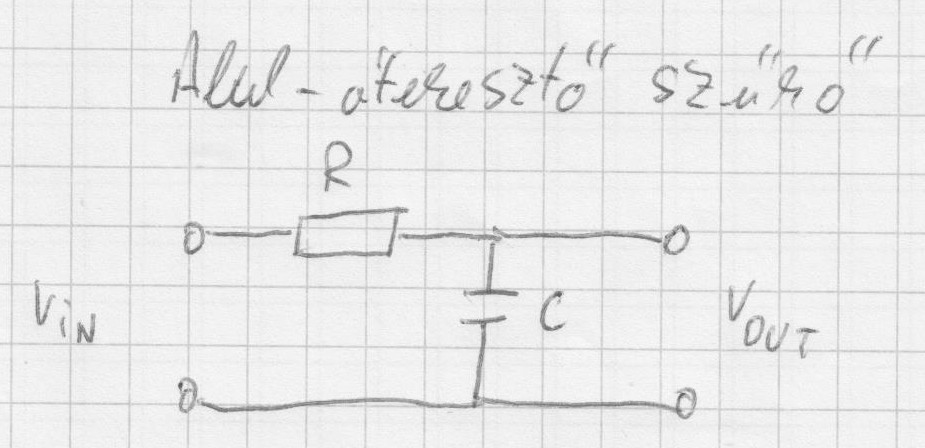
\includegraphics[scale=0.25]{figures/szuro_lp_rc.jpg}
    \caption{Alul-áteresztő szűrő}
\end{figure}

\subsection{Frekvencia, amplitúdó és fáziskarakterisztikák}

Frekvencia karakterisztikák: áteresztő tartománybeli erősítés ingadozás, átmeneti tartomány meredeksége, zárótartományi csillapítás ingadozás.

\begin{figure}[H]
    \centering
    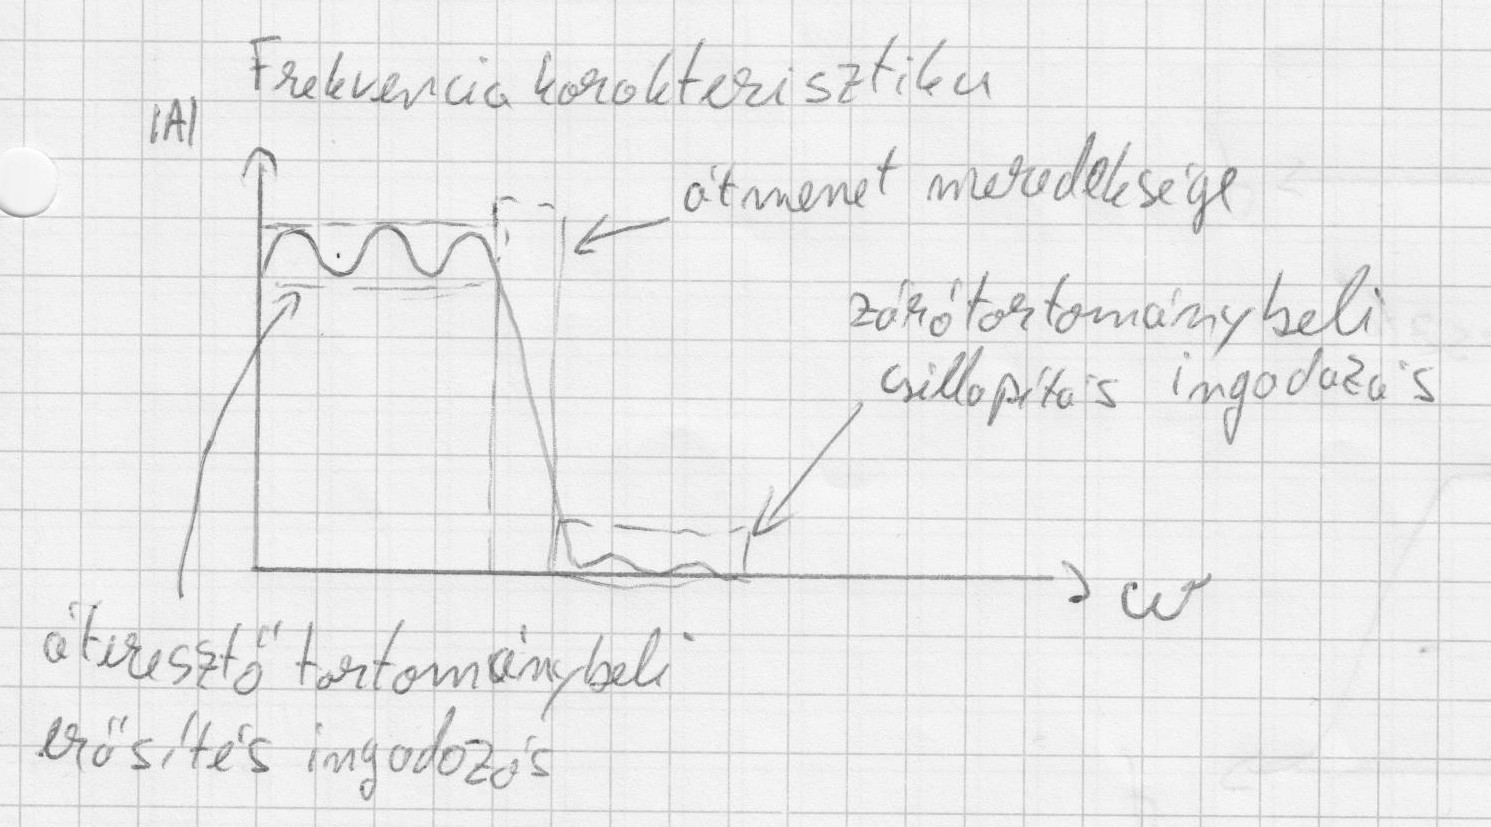
\includegraphics[scale=0.25]{figures/szuro_frekv.jpg}
    \caption{Frekvenciakarakterisztika}
\end{figure}

Fáziskarakterisztikák: fázismenet, csoportfutási idő. Fázismenet lehet lineáris vagy nemlineáris. Lineáris esetén minden frekvenciakomponenst ugyanannyit késleltet a szűrő. A csoportfutási idő a fázismenet frekvencia szerinti deriváltja.

\begin{figure}[H]
    \centering
    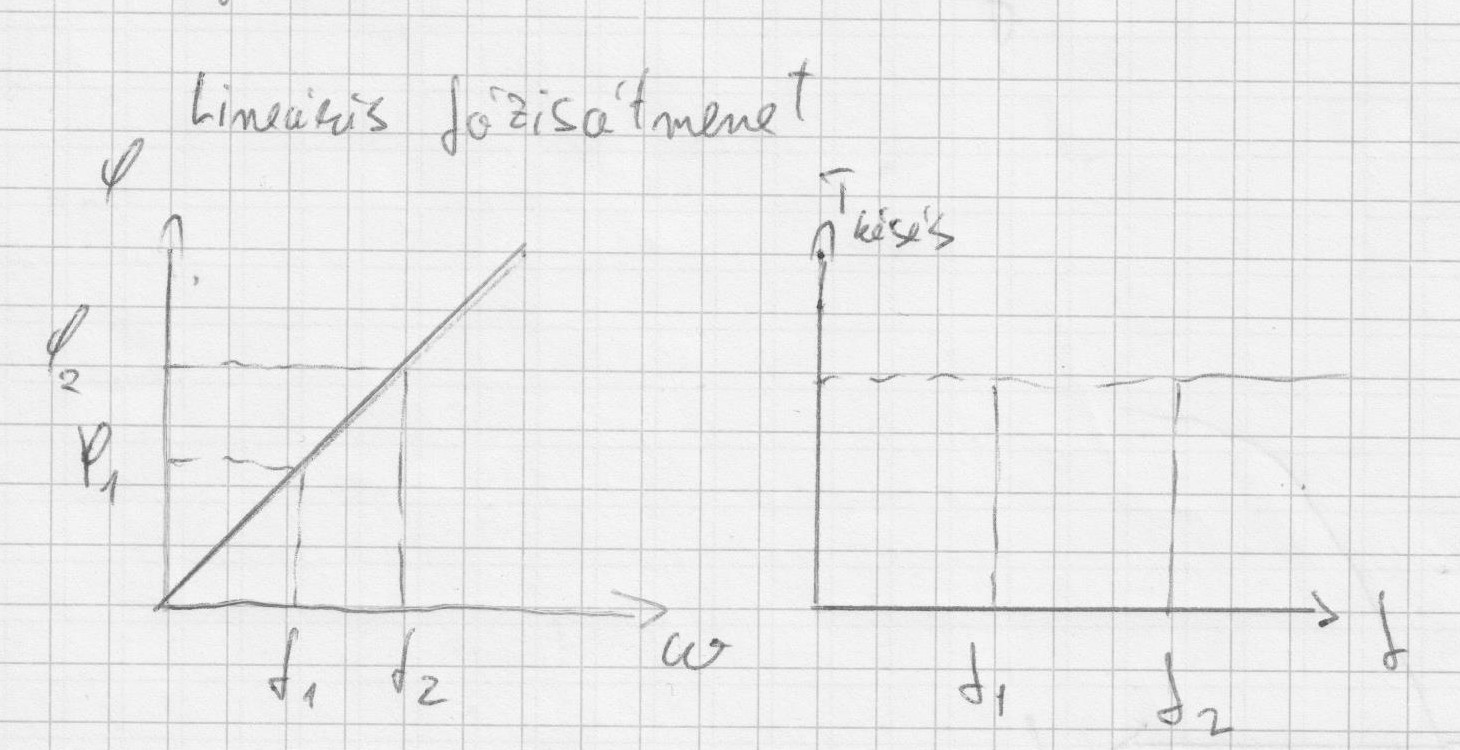
\includegraphics[scale=0.25]{figures/szuro_lin_menet.jpg}
    \caption{Lineáris fázismenet}
\end{figure}

\begin{figure}[H]
    \centering
    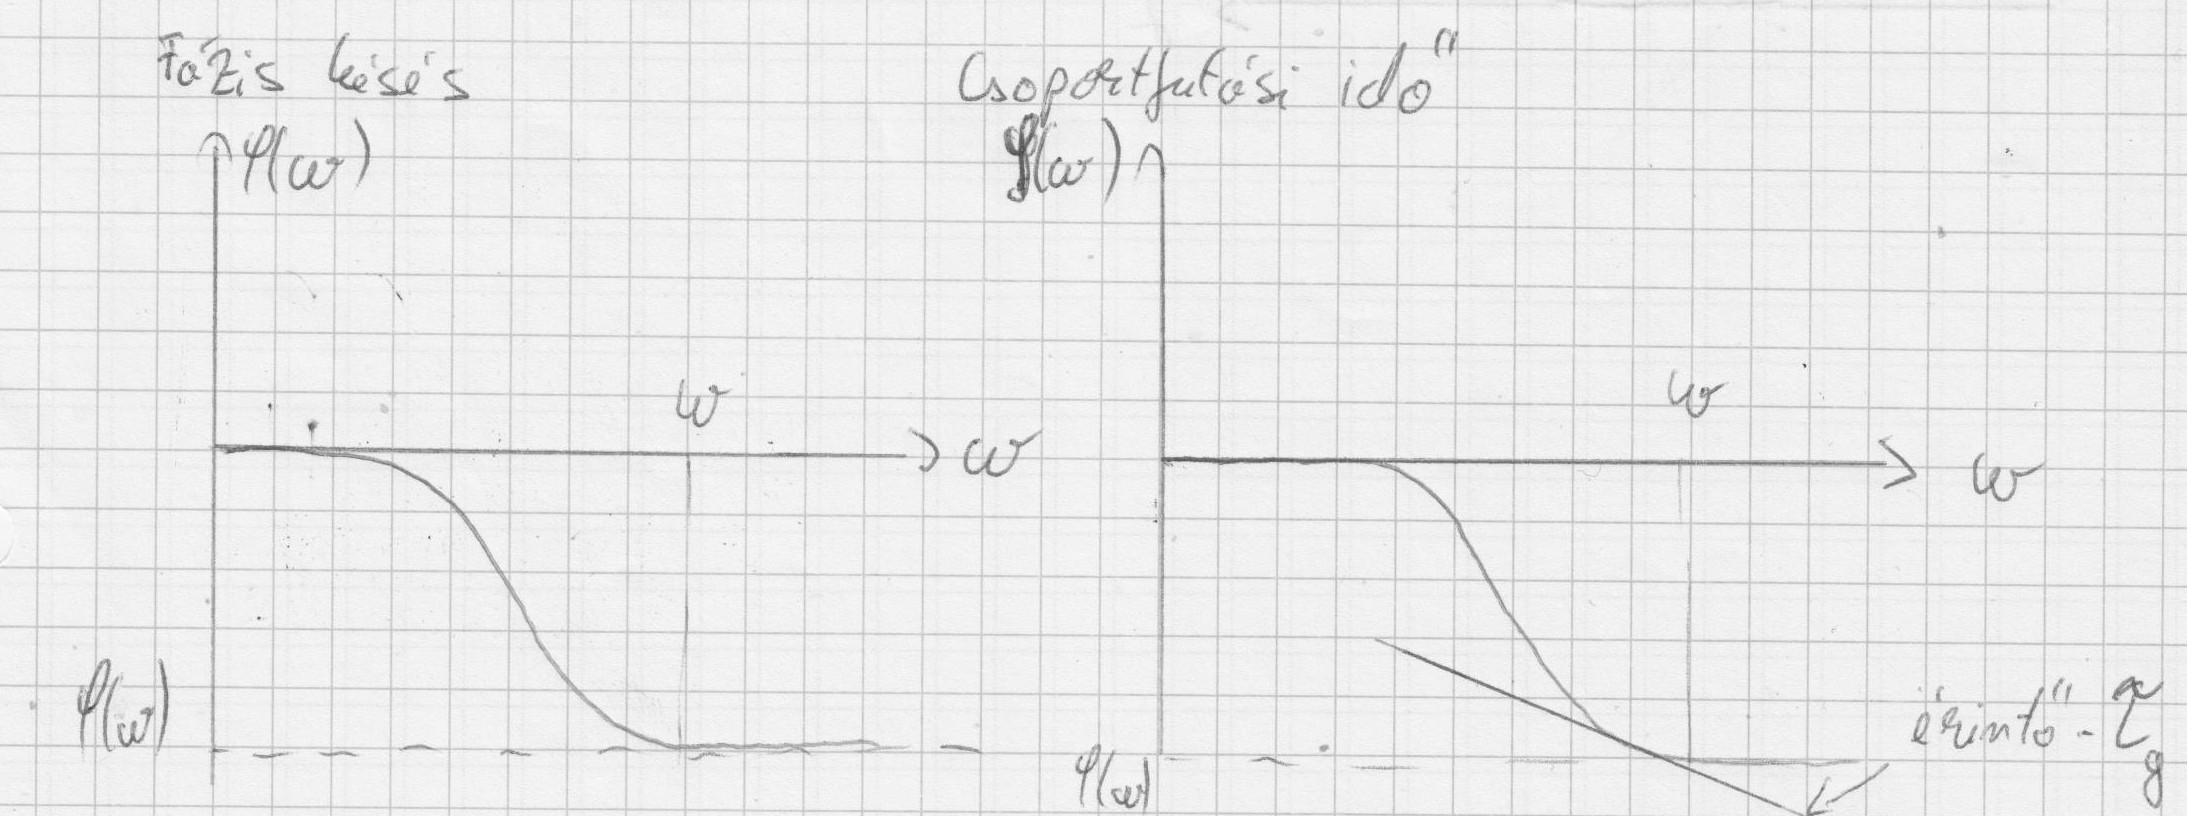
\includegraphics[scale=0.20]{figures/szuro_faz_csoport.jpg}
    \caption{Fáziskésés és csoportfutási idő}
\end{figure}

\begin{itemize}
    \item Fáziskésés: $\tau_{p}(w) = \frac{\varphi(w)}{w} $
    \item Csoportfutási idő: $\tau_{g}=\frac{d\varphi(w)}{dw}$
\end{itemize}


\subsection{Szűrő válaszának skálázása}

Az analóg szűrőknek az átviteli függvényük $f_{c} = 1$-re vannak normalizálva. Ahhoz, hogy a kívánt frekvenciánál legyen a vágás, szükséges, hogy a következő képlet szerint számoljuk ki az átviteli függvényt: $H_{w_{c}}(s) = \frac{k * \Pi_{i=1}^{n}(s - w_{c} * z_{i})}{w_{c}^{m - n} \Pi_{j=1}^{n} (s - w_{c}*p_{j})}$

\begin{itemize}
    \item $w_{c}$: vágási körfrekvencia
    \item $k$: erősítés
    \item $z_{i}$: zérusok
    \item $p_{j}$: pólusok
\end{itemize}

\subsection{Ábrázolási módok}

Hasznos az ábrázolási módot úgy végezni, hogy az áteresztőtartományban lineáris a skála (nagy felbontás), és a zárótartományban logaritmikus. Frekvencia tartományban ábrázoljuk a szűrőket, mert ott látható, hogy a szűrő melyik frekvenciákat engedi át és melyikeket nem.

\subsection{Szűrőtípusok közötti transzformációk}

Egy jól megtervezett alul-áteresztő szűrőből egy behelyettesítés elvégzése által lehet felül-áteresztő, sáváteresztő és sávzáró szűrőt kapni.

Felül-áteresztő: $H_{FE}: s \rightarrow \frac{1}{s}$

\begin{figure}[H]
    \centering
    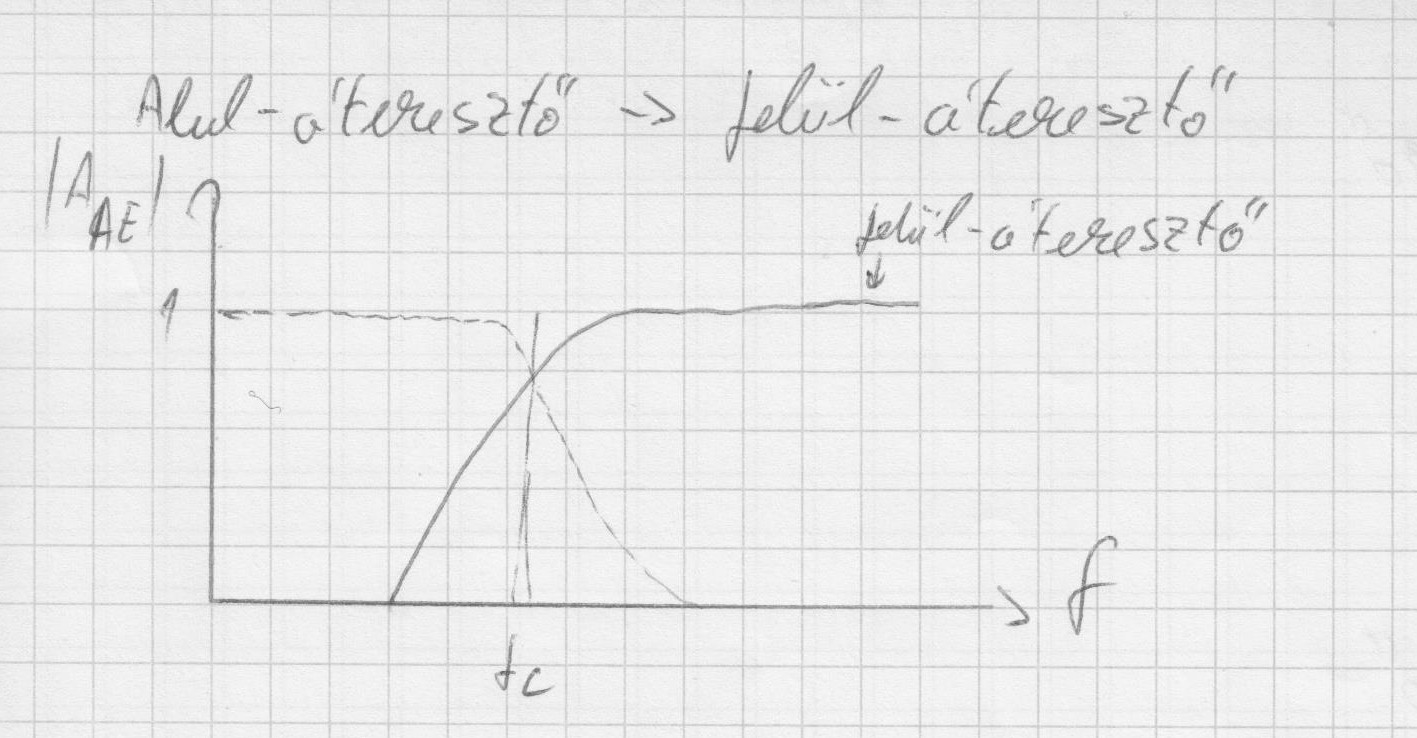
\includegraphics[scale=0.2]{figures/szuro_hp.jpg}
    \caption{Felül-áteresztő szűrő}
\end{figure}

Keskeny sávú sáváteresztő: $H_{SA}: s \rightarrow s - \frac{1}{s}$

\begin{figure}[H]
    \centering
    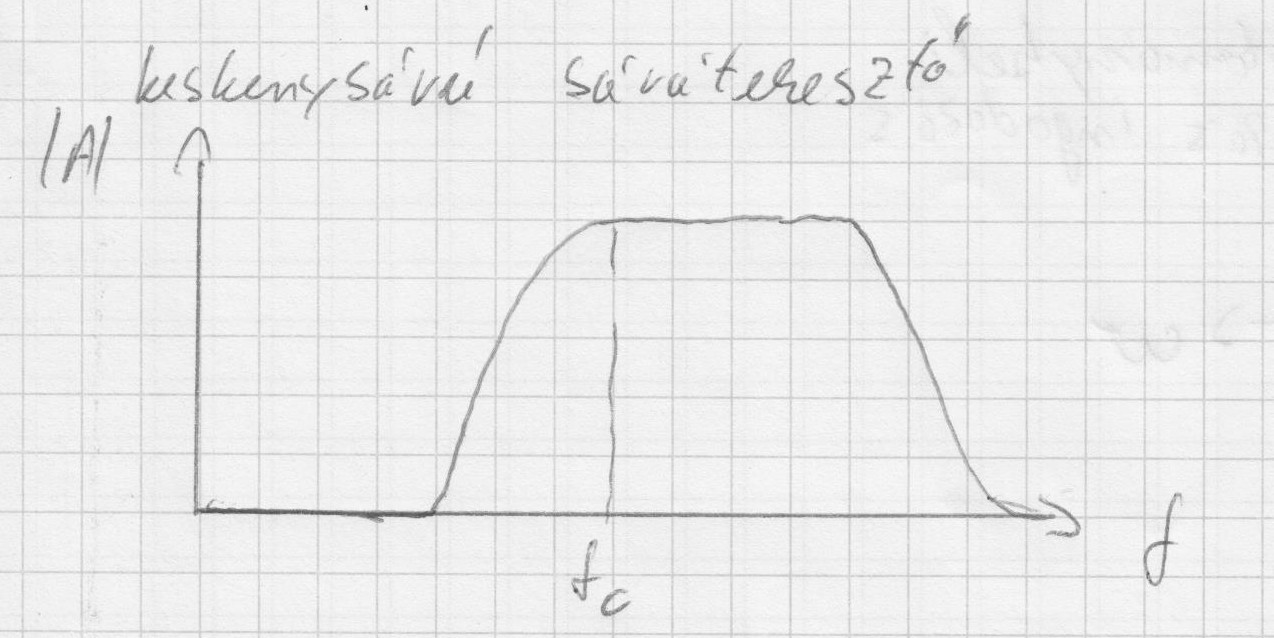
\includegraphics[scale=0.2]{figures/szuro_bp_good.jpg}
    \caption{Keskeny sávú sáváteresztő}
\end{figure}

Sáváteresztőt lehet egy alul-áteresztő és felül-áteresztő szűrő egymás utáni kapcsolásával is megvalósítani. Ez viszont behoz egy nem kívánt csillapítást az áteresztő tartományban.

\begin{figure}[H]
    \centering
    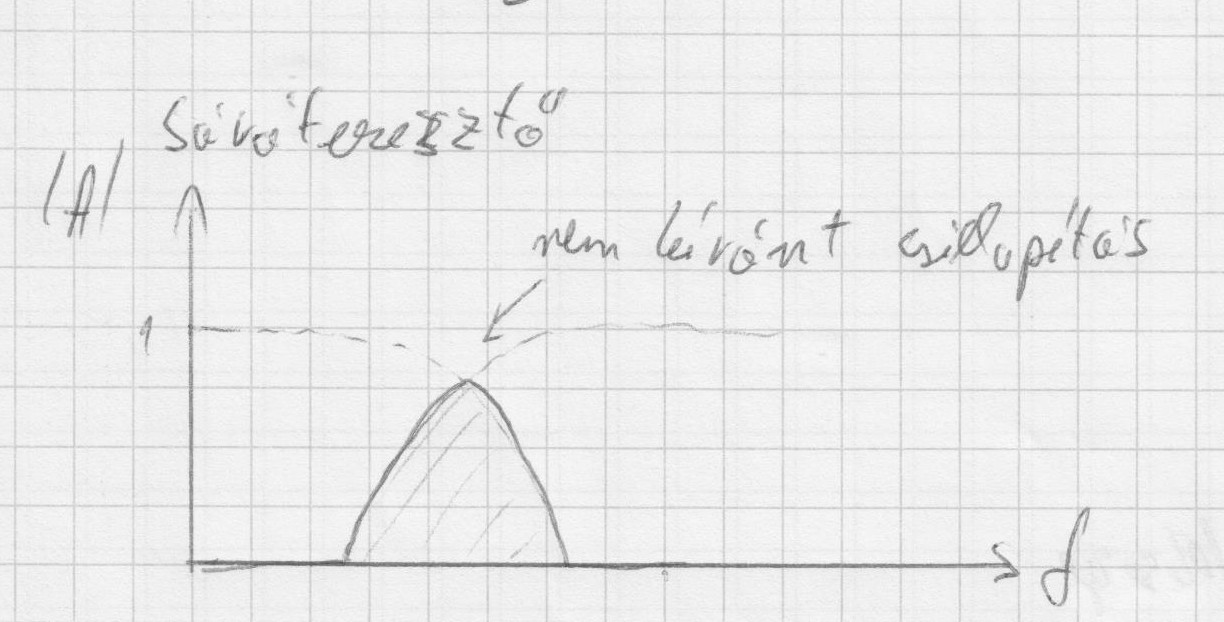
\includegraphics[scale=0.2]{figures/szuro_bp.jpg}
    \caption{Sáváteresztő: AE + FE szűrő kapcsolás}
\end{figure}

Sávzáró: $H_{SZ}: s \rightarrow \frac{s}{s^{2} - 1}$

\begin{figure}[H]
    \centering
    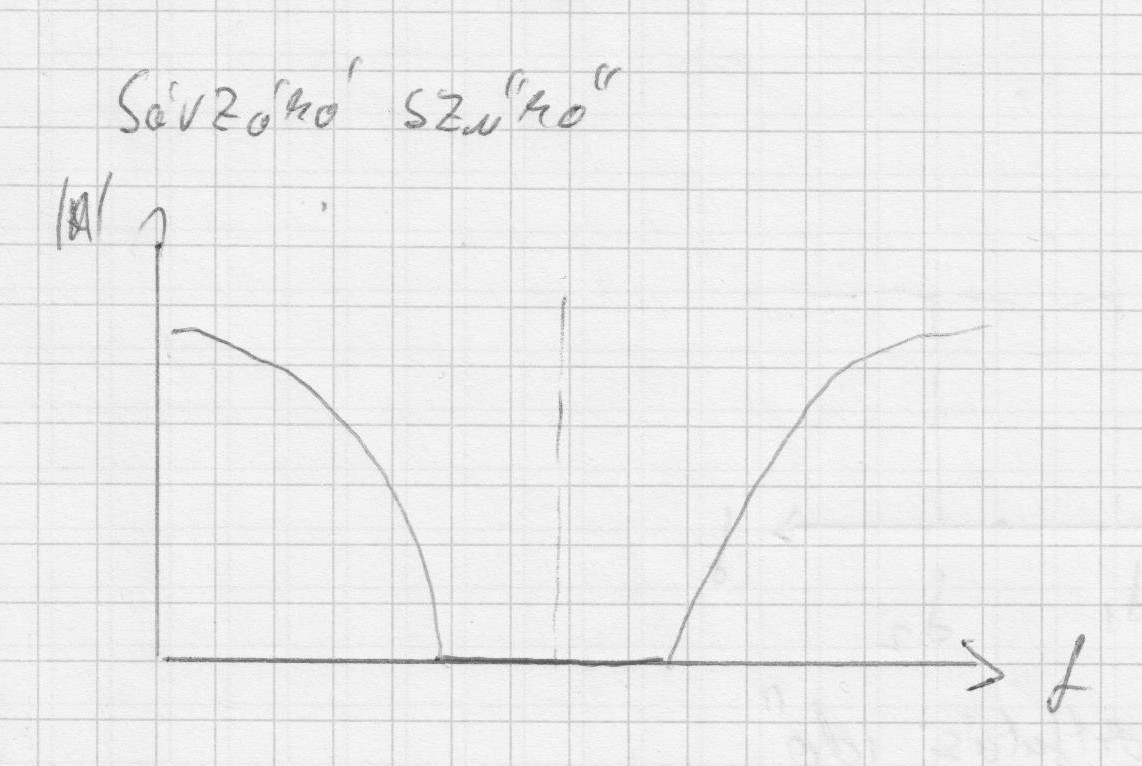
\includegraphics[scale=0.2]{figures/szuro_bs.jpg}
    \caption{Sávzáró szűrő}
\end{figure}


\section{3. Feladat}
\subsection{Súlyfüggvény kiszámítása}
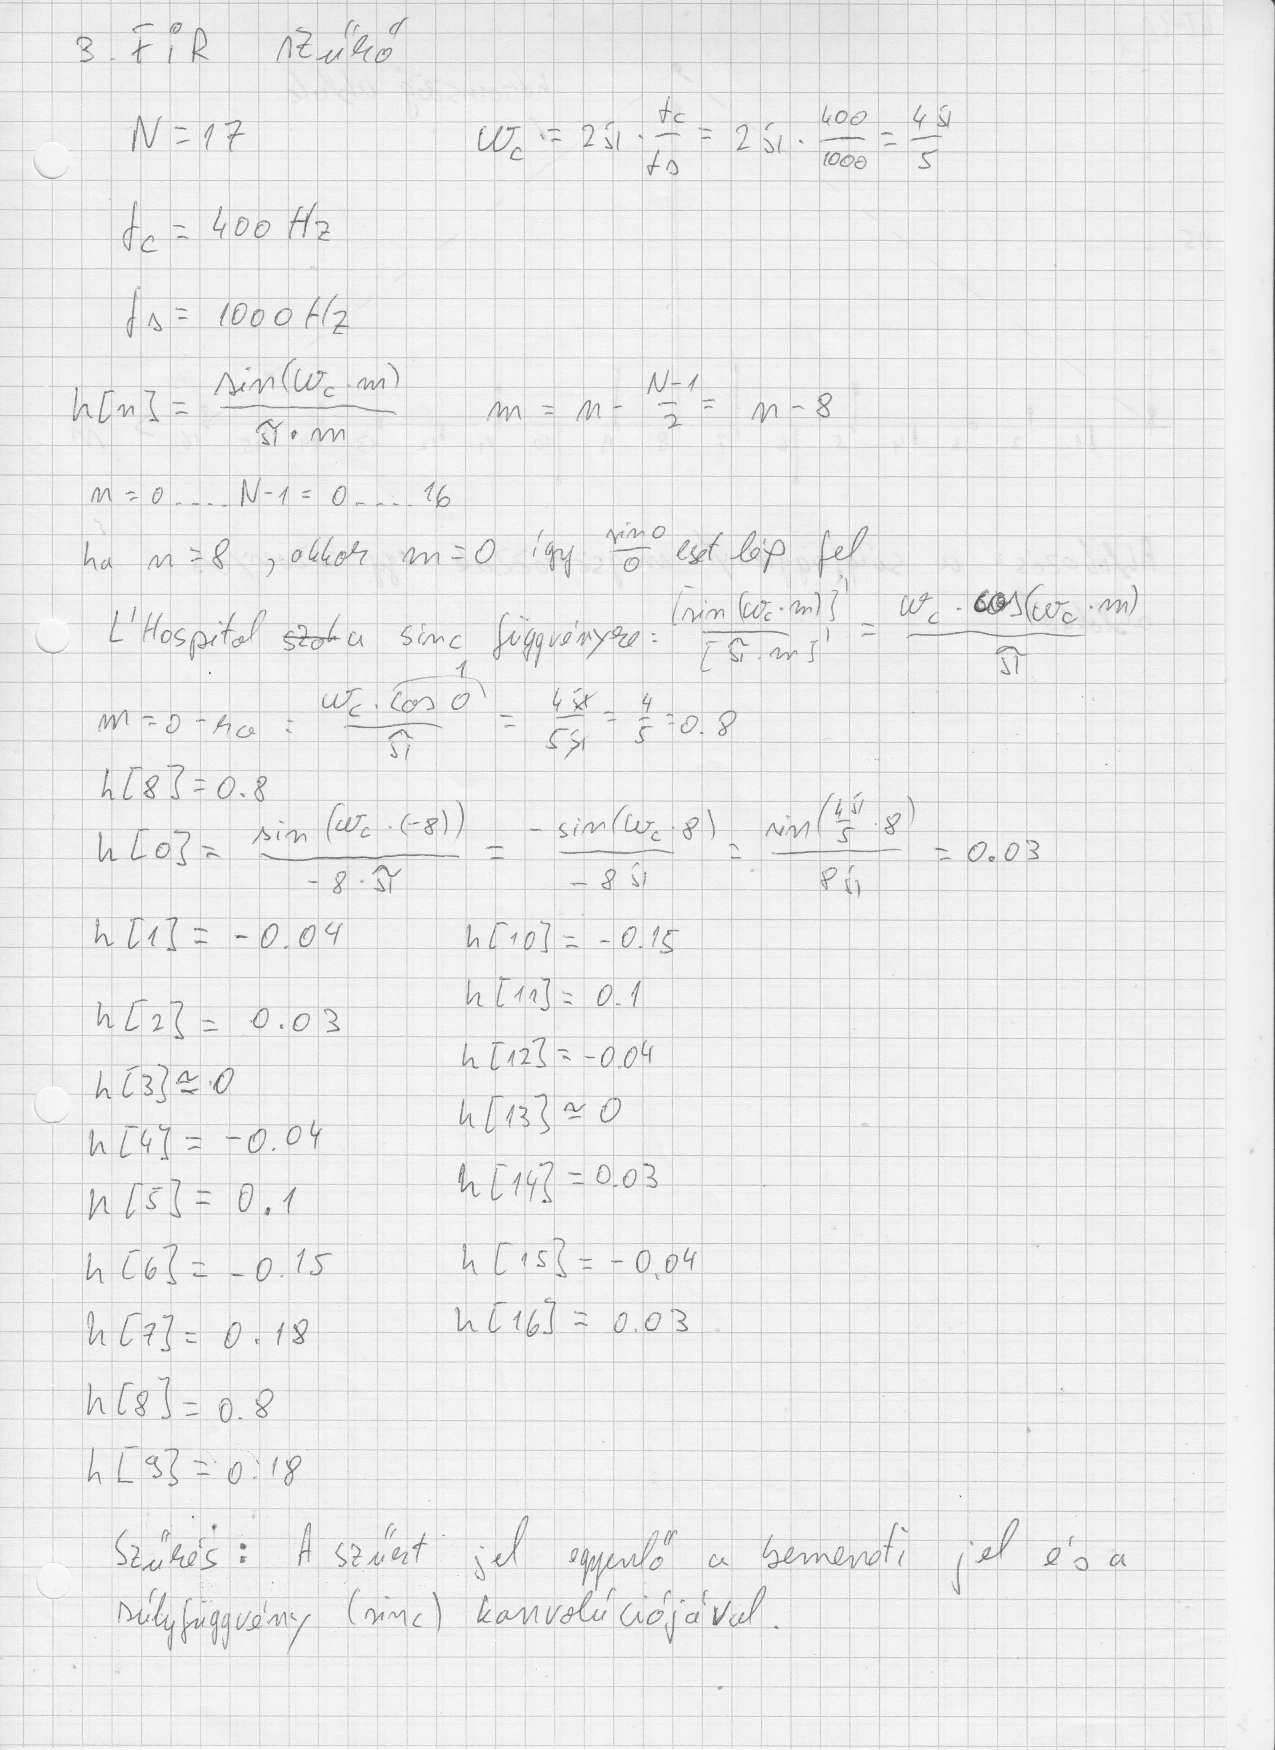
\includepdf[pages=-]{pdfs/fir.pdf}

\subsection{Python rész}

\subsubsection{Súlyfüggvény}

A következő ábrán látható a FIR szűrő súlyfüggvénye, a háromszög ablak és az ablakozás elvégzése utáni súlyfüggvény. Az ablakozás a súlyfüggvény beszorzása egy adott függvénnyel. Egyes típusú FIR szűrő, mivel páratlan a súlyfüggvény nem nulla elemeinek száma (N=17) és a súlyfüggvény szimmetrikus.

\begin{figure}[H]
    \centering
    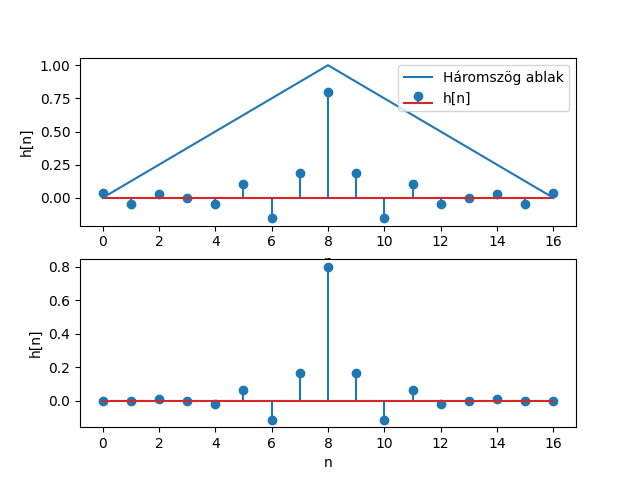
\includegraphics[scale=0.5]{figures/h.png}
    \caption{FIR súlyfüggvény, háromszög ablakkal}
\end{figure}

\subsubsection{Szűrés}

FIR szűrőnél a szűrt érték kiszámítható a bemeneti jel és a FIR súlyfüggvényének konvolúciójaként. Az alábbi ábrán látható egy 10 Hz-es és 470 Hz-es szinusz jel, ezek összege és a jel spektruma:

\begin{figure}[H]
    \centering
    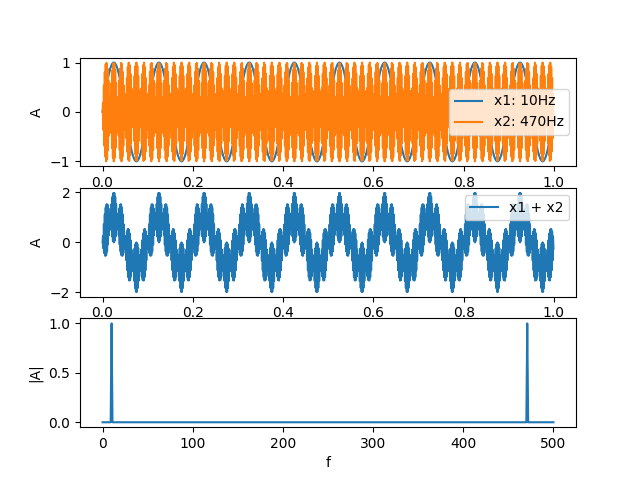
\includegraphics[scale=0.5]{figures/fir_sin.png}
    \caption{Bemeneti jel, két szinusz összege}
\end{figure}

A konvolúció elvégzése után a 470 Hz-es szinusz jelt ki sikerült szűrni: 

\begin{figure}[H]
    \centering
    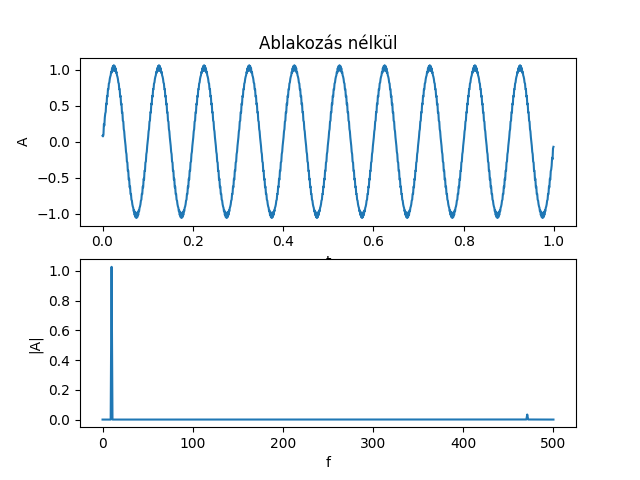
\includegraphics[scale=0.5]{figures/fir_no_win.png}
    \caption{Szűrés eredménye}
\end{figure}


\section{4. Feladat}
\subsection{Számolások}
\includepdf[pages=-]{pdfs/iir.pdf}

\subsection{Python ellenőrzés}

A kézzel számolt értékeket bevezettem Python-ba és kirajzoltam az átviteli függvény Bode diagramját. Az összehasonlításért a Scipy modult használva kirajzoltam a modul által tervezett szűrő Bode diagramját.

\begin{figure}[H]
    \centering
    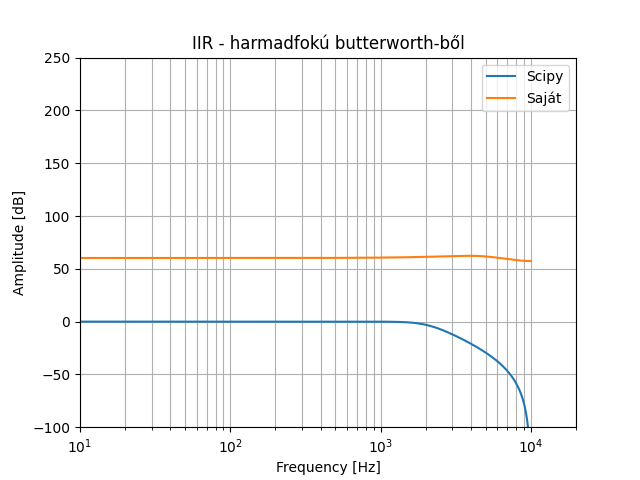
\includegraphics[scale=0.5]{figures/bode.png}
    \caption{Bode diagram kiszámolt és Scipy által tervezett IIR}
\end{figure}


A kézzel tervezett szűrő közel sem áll egy alul-áteresztő szűrőhöz. A számításokat többször leellenőriztem, viszont nem kaptam hibát. Mivel az IIR szűrőnél stabilitásprobléma léphet fel, úgy véltem az lehet a probléma. Kirajzoltam a rendszer pólusait és azt láttam, hogy ez valóban instabil (az egyik pólus az egységsugarú körön kívül van).

\begin{figure}[H]
    \centering
    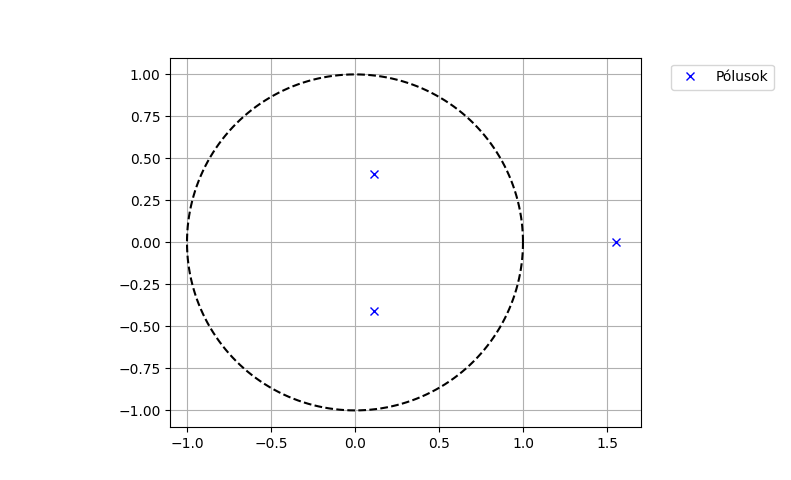
\includegraphics[scale=0.5]{figures/poles.png}
    \caption{Stabilitás vizsgálata}
\end{figure}



\appendix
\input{sections/anex.tex}


\end{document}